\section{Outils mis en place}

\begin{itemize}
	\item Site web en ligne (CMS Wordpress): \url{http://www.ecole.ensicaen.fr/~lvimont/} 

		\begin{figure}[h!]
			\centering
			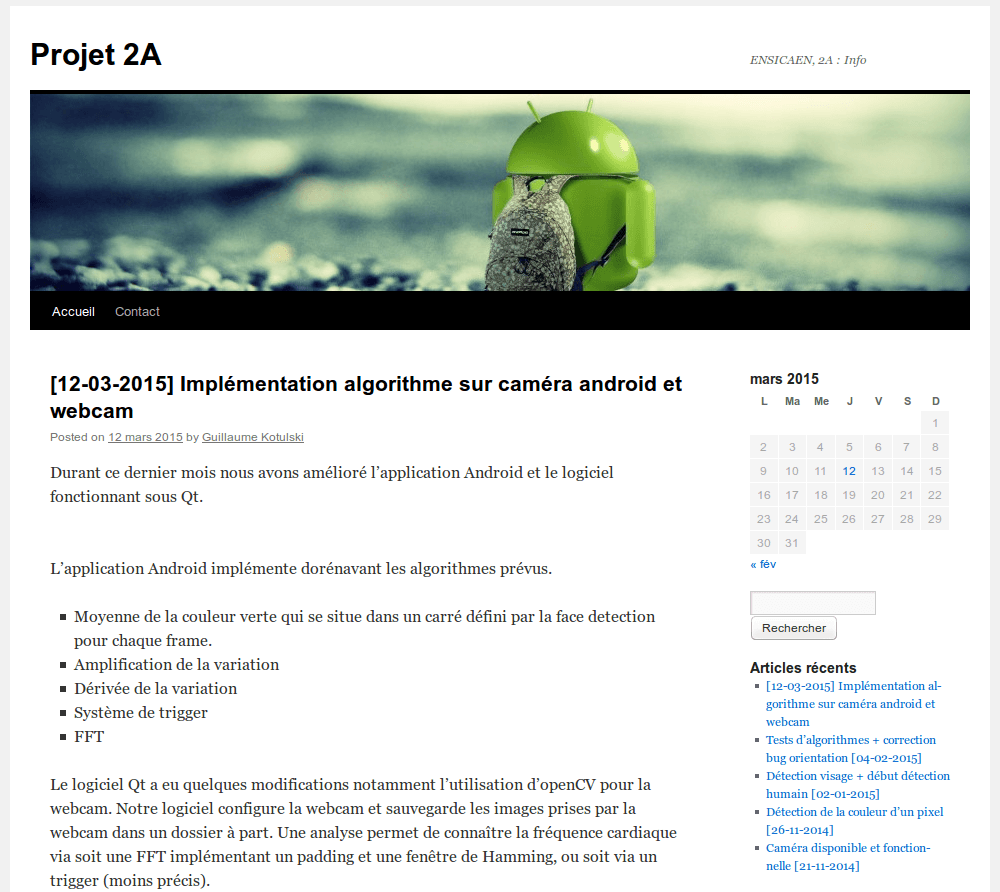
\includegraphics[width=0.9\textwidth]{data/website.png}
			\caption{Capture d'écran du site web.}
		\end{figure}

	\item Gestionnaire de versions (Git) 
		\begin{itemize}[label=\textbullet]
			\item Application Android: \url{https://github.com/F4r3n/Vamp} 
			\item Logiciel de traitement d'images: \url{https://github.com/F4r3n/ImageProject.git} 
		\end{itemize}
	\item Gestionnaire de projet (Trello)
\end{itemize}

\section{Technologies utilisées}

\begin{itemize}[label=\textbullet]
	\item QT:Nous avons utilisé la librairie Qt pour pouvoir créer notre application qui permettait de tester les algorithmes.
	\item Android:La programmation sous Android s'est faite en utilisant Java et de l'XML.
	\item OpenCV:Utilisation de la webcam et application utilisant la caméra gérée  par OpenCV
	\item Pyhton: Traitement des données pour création d'un graphique et permet une meilleure vérification des résultats
\end{itemize}

\section{Algorithme mis en place}

L’œil humain est limité, en effet il est incapable de voir les subtils changements temporels. Alors
que justement en effectuant des traitements sur une vidéo. On est capable de révéler ces changements
comme par exemple, la circulation du sang. On peut même grâce à ça réussir à connaître le pouls d'une
personne.
\\
De plus lorsque le sang monte jusqu'à la tête puis descend, il fait que notre tête bouge imperceptiblement, ces différents changements peuvent capturés avec un téléphone portable.
\\
Mais comment obtenir ces changements ? Comment savoir où se situe le visage ?\\

 Dans un premier temps nous devons détecter si quelque chose ayant un visage humain se tenait devant l'appareil, ceci se fait très bien par l'api de Google sur Android et même par OpenCV.
 Après détection de la personne nous pouvons obtenir des coordonnées nous disant où se situe le visage.\\
 Maintenant que nous savons où se situe le visage, nous nous demandons comment reconnaître une fréquence ?\\
 Nous avons choisi l'espace de couleur RGB car c'est dans cette espace de couleur que nous détectons le plus de variations, les autres modes tel que HSL ou HUV nous donnaient des valeurs plus faibles.
 Nous avons donc fait une moyenne du canal vert (c'est le canal vert qui varie le plus) pour chaque pixel se situant dans un rectangle (en l’occurrence le rectangle délimitant le visage).
 Et ceci pour chaque frame que l'on capturait, nous obtenions une certaine valeur.
 Après obtention de ces valeurs nous pouvions les traiter.
 La variation des valeurs étant très grande, nous avons dans un premier temps fait une moyenne glissante. Puis pour amplifier les variations nous avons avons fait une dérivée de Taylor.
 Nos valeurs étant prêtes à être analyser, nous les avons analyser de deux façons différentes.
 La première, la plus simple fut le Trigger, qui nous permettait d'avoir une fourchette de pulsation.\\ La deuxième plus longue,une FFT, nécessitait des étapes de calcul supplémentaire tel que un fenêtrage de Hamming et un padding, mais donnait des résultats plus précis.
 \\
 Ces deux analyses nous permettait d'avoir le pouls de notre utilisateur (dans le cas idéal).
 \\ 

Nous avons remarqué que la collecte des données n'accentuait pas assez les variations, nous avons donc créé une deuxième méthode qui en restant basé sur le même principe que la première technique, nous découpions notre image
par zone de petits carrés de pixels. Par exemple une zone serait d'une taille de 5*5. On réalise 
ainsi une moyenne de chaque zone, puis par la suite une moyenne de ces moyennes. Enfin on rapplique
les mêmes fonctions citées précédemment.

\section{Solutions mis en place}

Durant le projet nous avons développés plusieurs outils pour répondre au besoin. Une application Android qui permettrait d'utiliser le moyen d'authentification désiré et ainsi déverrouiller le smartphone d'une
personne. Un logiciel C++ utilisant la librairie QT a également été mis en place, afin de pouvoir tester plus facilement les algorithmes que nous voulions développer. Dans la suite du projet, il a également
permis d'utiliser la webcam. 

\subsection{Développement Android}

	Notre application Android est capable d'utiliser la caméra frontale de n'importe quel smartphone. L'api d'Android propose une classe appelée FaceDetectionListener qui va permettre de capter, les visages présent 
	devant une caméra, grâce à ce système il est possible de dessiner un Rect (c'est à dire un rectangle) autour du visage de la personne. C'est notre classe DisplayedFace qui se charge de ce travail. Une fois la 
	reconnaissance mis en place, nous avons utiliser la fonction \href{http://developer.android.com/reference/android/hardware/Camera.PreviewCallback.html#onPreviewFrame\%28byte\%5B\%5D,\%20android.hardware.Camera\%29}{onPreviewFrame}. Cette dernière permet d'enregistrer en temps réel, les données. On lance un compteur quand la première reconnaissance d'un visage a lieu, ce dernier va durer 5 secondes.\\
\\
	Les données ainsi récoltées sont au format de l'espace de couleur \href{http://fr.wikipedia.org/wiki/YUV}{YUV}. Nous devons donc convertir ces données au format RGB qui se révèle plus évocateur au niveau des variations. 
	A la fin du compteur, on réalise une dérivée, puis une amplification des valeurs obtenues. On observe alors les variations qu'on obtient et on conclu alors sur la présence ou non d'un humain.
	\\
	\\
	L'api de Google est très rapide pour détecter un visage et pour nous fournir ces coordonnées en faisant très peu de calcul. Mais celle-ci ne suit pas les petits changements de position, par exemple lorsque l'utilisateur prend une vidéo il bouge légèrement ce qui peut changer le résultat final.
	\\
	\\
	Pour résoudre ce manque nous avons codé une application fonctionnant avec OpenCV, celle-ci suit parfaitement le visage lorsqu'il bouge. Mais le temps de traitement d'une image par OpenCV est beaucoup plus lent que l'api de Google. Ce qui fait que nous tournons à environ 7 FPS en back-caméra et 2 FPS en front-caméra ce qui n'est pas idéal.
	\begin{figure}[h!]
			\centering
			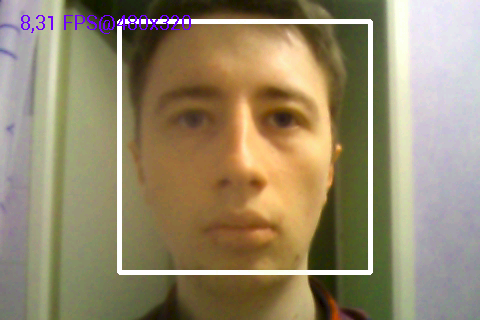
\includegraphics[width=0.9\textwidth]{data/opencv.png}
			\caption{Aperçu de l'application OpenCV}
		\end{figure}
	\\
	\\
	L'application sous OpenCV permet de faire une FFT et un système de Trigger, en croisant les résultats donnés par ces deux systèmes nous obtenons un meilleur résultat que si il n'y avait seulement le Trigger.  

\subsection{Développement C++}

	Nous avons créé un logiciel C++ nous permettant de tester nos algorithmes avant de les implémenter sous Android.
	Ce logiciel a de nombreuses fonctionnalités, notamment le découpage d'une vidéo en images pour permettre une analyse plus poussée.
	Nous utilisons avconv qui permet de découper une vidéo de n'importe quelle taille en une multitude d'images (15 images * taille de la vidéo)
	Après avoir découpé la vidéo en images nous faisons une analyse sur ces images.
	Cette analyse se découpe en plusieurs étapes.
	Dans un premier temps nous dessinons un rectangle autour d'un visage (si la fonction du rectangle automatique n'est pas enclenchée)
	Puis nous choisissons le type d'analyse a effectué, il y en a deux types:\\
		-L'une fait la moyenne de tous les pixels qui se situe dans le carré\\
		-La seconde découpe le rectangle en plusieurs zones de 5*5 puis amplifie les variations et fait une moyenne des valeurs
	Après avoir lancé l'analyse, nous affichons les courbes ainsi obtenues par notre application.\\

	Nous pouvons voir la FFT, l'amplification, la dérivée ou une combinaison de plusieurs méthodes.
	L'amplification utilise la dérivée de Taylor du premier degré.
	La FFT utilise un filtre passe-bas combiné avec une fenêtre de Hamming et un padding.
	La FFT permet de connaître le rythme cardiaque d'une personne de manière précise si l'image est assez stable.
	Nous avons créé un Trigger qui permet aussi de connaître la fréquence cardiaque d'une personne mais de manière moins précise, le Trigger nous donne une fourchette de valeurs.\\

	Si l'espace de couleur que nous avons choisi ne donne pas des résultats corrects nous pouvons en choisir un autre.
	Nous avons différents espaces de couleur disponible dont RGB, HSL, HUV et nous pouvons lancer une analyse avec un espace de couleur différent de RGB.\\

	Les analyses avec des vidéos classiques n'étant pas suffisantes pour nos tests, nous avons dû faire une analyse avec des vidéos de la webcam.
	La webcam est configurée et lancée via la librairie OpenCV et nous enregistrons les images de la webcam avec une fréquence de 15 frames pas seconde.\\

\section{Problèmes rencontrés}

\subsection{Limitation des sessions à l'ENSICAEN}

Lors du projet, nous avons rencontrés de nombreux problèmes. L'un des plus embêtant est la limite des sessions à l'Ensicaen. En effet, nos sessions dispose du taille limité, nous pouvons uniquement travailler sous Windows (car
c'est seulement sous cet environnement que sont installés les outils Android) hors nous disposons d'uniquement 150 Mo, or rien qu'avec Firefox, si nous ne nettoyons par régulièrement l'historique, la session se retrouve 
complète. Nous avons malheureusement expérimenté le soucis et perdu ainsi, une après midi de travail. 

\subsection{Problèmes rencontrés lors du développement Android}

Nous avons eu un problème de rotation, les coordonnées que l'on converser se révélait mauvaise. On avait en effet un problème de rotation, afin d'éviter cela on force le mode portrait.

La première version de notre application était capable d'enregistrer 15 frames par seconde, or au final on obtenait seulement une trentaine de valeurs, cela était du à la conversion du format YUV au format RGB que l'on 
effectuer à chaque fois que nous rentrons dans la fonction onPreviewFrame, comme la conversion est coûteuse O(n\up{2}), on perdait des valeurs. Pour optimiser, le nombre de valeurs nous effectuons maintenant la conversion
une fois le timer fini. On réalise alors dans la boucle une simple sauvegarde des données bruts. 
Toutefois cette méthode, nous a causé pas mal de soucis, notamment des out of memory, c'est à dire, que nous réalisions une allocation trop grande par rapport à la mémoire disponible \ldots{}
\\
Même si l'algorithme fonctionnait avec des vidéos, ceci ne voulait pas dire qu'il fonctionnerait sous Android.
En effet lorsque avec la caméra on se prend en vidéo on bouge légèrement, ce qui pose de nombreux problèmes de stabilité. 
Les variations que nous obtenons alors ne seraient plus celle de la pulsation mais celles du mouvement régulier de la main.

% L'incompétence des chercheurs

